\documentclass[aspectratio=169]{beamer}

% Theme and Color Setup
\usetheme{Madrid}
\usecolortheme{whale}
\useinnertheme{rectangles}
\useoutertheme{miniframes}

% Additional Packages
\usepackage[utf8]{inputenc}
\usepackage[T1]{fontenc}
\usepackage{graphicx}
\usepackage{booktabs}
\usepackage{listings}
\usepackage{amsmath}
\usepackage{amssymb}
\usepackage{xcolor}
\usepackage{tikz}
\usepackage{pgfplots}
\pgfplotsset{compat=1.18}
\usetikzlibrary{positioning}
\usepackage{hyperref}

% Custom Colors
\definecolor{myblue}{RGB}{31, 73, 125}
\definecolor{mygray}{RGB}{100, 100, 100}
\definecolor{mygreen}{RGB}{0, 128, 0}
\definecolor{myorange}{RGB}{230, 126, 34}
\definecolor{mycodebackground}{RGB}{245, 245, 245}

% Set Theme Colors
\setbeamercolor{structure}{fg=myblue}
\setbeamercolor{frametitle}{fg=white, bg=myblue}
\setbeamercolor{title}{fg=myblue}
\setbeamercolor{section in toc}{fg=myblue}
\setbeamercolor{item projected}{fg=white, bg=myblue}
\setbeamercolor{block title}{bg=myblue!20, fg=myblue}
\setbeamercolor{block body}{bg=myblue!10}
\setbeamercolor{alerted text}{fg=myorange}

% Set Fonts
\setbeamerfont{title}{size=\Large, series=\bfseries}
\setbeamerfont{frametitle}{size=\large, series=\bfseries}
\setbeamerfont{caption}{size=\small}
\setbeamerfont{footnote}{size=\tiny}

% Footer and Navigation Setup
\setbeamertemplate{footline}{
  \leavevmode%
  \hbox{%
  \begin{beamercolorbox}[wd=.3\paperwidth,ht=2.25ex,dp=1ex,center]{author in head/foot}%
    \usebeamerfont{author in head/foot}\insertshortauthor
  \end{beamercolorbox}%
  \begin{beamercolorbox}[wd=.5\paperwidth,ht=2.25ex,dp=1ex,center]{title in head/foot}%
    \usebeamerfont{title in head/foot}\insertshorttitle
  \end{beamercolorbox}%
  \begin{beamercolorbox}[wd=.2\paperwidth,ht=2.25ex,dp=1ex,center]{date in head/foot}%
    \usebeamerfont{date in head/foot}
    \insertframenumber{} / \inserttotalframenumber
  \end{beamercolorbox}}%
  \vskip0pt%
}

% Turn off navigation symbols
\setbeamertemplate{navigation symbols}{}

% Title Page Information
\title[Week 8: Hadoop Ecosystem]{Week 8: Hadoop Ecosystem}
\author[J. Smith]{John Smith, Ph.D.}
\institute[University Name]{
  Department of Computer Science\\
  University Name\\
  \vspace{0.3cm}
  Email: email@university.edu\\
  Website: www.university.edu
}
\date{\today}

% Document Start
\begin{document}

\frame{\titlepage}

\begin{frame}[fragile]
    \frametitle{Introduction to Hadoop Ecosystem}
    \begin{block}{Overview}
        Overview of the Hadoop Ecosystem and its significance in handling large-scale data processing.
    \end{block}
\end{frame}

\begin{frame}[fragile]
    \frametitle{1. What is the Hadoop Ecosystem?}
    \begin{itemize}
        \item A set of tools and technologies enabling storage, processing, and analysis of large datasets.
        \item Essential for handling \textbf{Big Data}, which is often too complex for traditional methods.
    \end{itemize}
\end{frame}

\begin{frame}[fragile]
    \frametitle{2. Key Components of the Hadoop Ecosystem}
    \begin{itemize}
        \item \textbf{Hadoop Common}: Essential libraries and utilities.
        \item \textbf{HDFS}: Distributed file system for high-throughput access to data.
        \item \textbf{YARN}: Resource management and job scheduling.
        \item \textbf{MapReduce}: Programming model for processing large datasets.
    \end{itemize}
\end{frame}

\begin{frame}[fragile]
    \frametitle{2. Key Components of the Hadoop Ecosystem (continued)}
    \begin{itemize}
        \item \textbf{Hadoop Ecosystem Tools}:
        \begin{itemize}
            \item \textbf{Apache Hive}: SQL-like query tool for data warehousing.
            \item \textbf{Apache Pig}: High-level language for dataset analysis.
            \item \textbf{Apache HBase}: NoSQL database on top of HDFS.
            \item \textbf{Apache Spark}: General-purpose cluster computing system.
            \item \textbf{Apache Flume}: Service for collecting log data.
            \item \textbf{Apache Sqoop}: Tool for data transfer between Hadoop and RDBMS.
        \end{itemize}
    \end{itemize}
\end{frame}

\begin{frame}[fragile]
    \frametitle{3. Significance of the Hadoop Ecosystem}
    \begin{itemize}
        \item \textbf{Scalability}: Can grow by adding more machines.
        \item \textbf{Cost-effective}: Utilizes commodity hardware.
        \item \textbf{Flexibility}: Supports multiple data formats.
        \item \textbf{Fault Tolerance}: Ensures data is replicated and recoverable.
    \end{itemize}
\end{frame}

\begin{frame}[fragile]
    \frametitle{4. Real-World Applications}
    \begin{itemize}
        \item \textbf{Social Media Analysis}: Targeted advertising strategies based on user data.
        \item \textbf{Healthcare}: Better diagnostics from processed patient data and medical images.
        \item \textbf{Retail Analytics}: Optimized sales strategies from processed shopping trends.
    \end{itemize}
\end{frame}

\begin{frame}[fragile]
    \frametitle{5. Diagram: Hadoop Ecosystem Overview}
    \begin{block}{Diagram Representation}
        A conceptual diagram illustrating the interaction between HDFS, YARN, and various processing tools, along with the data flow.
    \end{block}
\end{frame}

\begin{frame}[fragile]
    \frametitle{Key Points}
    \begin{itemize}
        \item Hadoop is an ecosystem of tools, not a single product.
        \item Offers flexibility, scalability, and cost-effectiveness for big data.
        \item Understanding the ecosystem is crucial for leveraging its full potential.
    \end{itemize}
\end{frame}

\begin{frame}[fragile]
    \frametitle{Conclusion}
    \begin{block}{Conclusion}
        The Hadoop Ecosystem is vital for managing and deriving insights from large volumes of data in the landscape of Big Data technology.
    \end{block}
\end{frame}

\begin{frame}[fragile]
    \frametitle{What is Hadoop? - Definition}
    
    \begin{block}{Definition of Hadoop}
        Hadoop is an open-source framework designed to store and process large datasets in a distributed computing environment. It allows users to scale their data processing capabilities by leveraging clusters of computers, making it a vital part of managing big data. 
    \end{block}

    \begin{block}{Purpose in Big Data}
        Hadoop addresses challenges associated with big data, such as:
        \begin{itemize}
            \item \textbf{Large Data Volumes}: Support for petabytes of data.
            \item \textbf{Data Variety}: Ability to process structured and unstructured data.
            \item \textbf{Velocity}: Fast processing of real-time data streams.
            \item \textbf{Veracity}: Reliable data storage and processing.
        \end{itemize}
    \end{block}
\end{frame}

\begin{frame}[fragile]
    \frametitle{What is Hadoop? - Key Components}

    \begin{block}{Key Components of Hadoop Ecosystem}
        Hadoop consists of several core components:
        \begin{itemize}
            \item \textbf{Hadoop Distributed File System (HDFS)}
                \begin{itemize}
                    \item Purpose: A distributed file system designed for high-throughput access and vast data storage.
                    \item Key Features:
                        \begin{itemize}
                            \item Data is split into blocks distributed across nodes.
                            \item Fault-tolerant through data replication (default is 3 copies).
                        \end{itemize}
                \end{itemize}
                
            \item \textbf{MapReduce}
                \begin{itemize}
                    \item Purpose: A programming model for processing large datasets with a parallel algorithm.
                    \item Functionality: Divides tasks into smaller sub-tasks (Map phase) and aggregates results (Reduce phase).
                    \item Example: Processing web server logs to aggregate hits per URL.
                \end{itemize}
                
            \item \textbf{Yet Another Resource Negotiator (YARN)}
                \begin{itemize}
                    \item Purpose: Resource management layer that allocates resources and manages job scheduling.
                    \item Key Features:
                        \begin{itemize}
                            \item Allows multiple data processing engines on the same cluster.
                            \item Enhances cluster utilization and resource sharing.
                        \end{itemize}
                \end{itemize}
        \end{itemize}
    \end{block}
\end{frame}

\begin{frame}[fragile]
    \frametitle{What is Hadoop? - Use Case and Conclusion}

    \begin{block}{Example Use Case}
        Consider an online retail company using Hadoop to analyze customer behavior:
        \begin{itemize}
            \item \textbf{Data Collection}: HDFS stores transaction data, reviews, and clickstream data.
            \item \textbf{Data Analysis}: MapReduce processes this data to generate insights on frequent purchase combinations.
            \item \textbf{Resource Management}: YARN manages simultaneous analytics jobs ensuring optimal performance.
        \end{itemize}
    \end{block}

    \begin{block}{Conclusion}
        Hadoop is a transformative technology for big data, enabling efficient management and analysis. Understanding its components helps realize its full potential in real-world applications, particularly in finance, retail, and telecommunications.
    \end{block}
\end{frame}

\begin{frame}[fragile]
    \frametitle{Key Components of Hadoop - Introduction}
    \begin{block}{Overview}
        Hadoop is an open-source framework designed for storing and processing large datasets in a distributed environment. The main components include:
    \end{block}
    \begin{enumerate}
        \item Hadoop Distributed File System (HDFS)
        \item MapReduce
        \item Yet Another Resource Negotiator (YARN)
    \end{enumerate}
\end{frame}

\begin{frame}[fragile]
    \frametitle{Key Component: Hadoop Distributed File System (HDFS)}
    \begin{block}{Overview}
        HDFS is the storage layer of Hadoop that stores large data sets across multiple machines efficiently.
    \end{block}
    \begin{itemize}
        \item **Scalability**: Easily add more hardware to accommodate growth.
        \item **Data Redundancy**: Default replication of each block is three times to ensure reliability.
        \item **High Throughput**: Optimized for large data reads over low-latency access.
    \end{itemize}
    \begin{block}{Example}
        In social media applications, user-generated data such as posts and comments are stored in HDFS, allowing the system to handle increased activity by adding more nodes.
    \end{block}
\end{frame}

\begin{frame}[fragile]
    \frametitle{Key Component: MapReduce}
    \begin{block}{Overview}
        MapReduce is the computational framework of Hadoop that processes large datasets in parallel.
    \end{block}
    \begin{enumerate}
        \item **Map Phase**: The input dataset is divided into smaller chunks, generating intermediate key-value pairs.
        \item **Reduce Phase**: The pairs are combined and aggregated to produce the final output.
    \end{enumerate}
    \begin{itemize}
        \item Ideal for batch processing and tasks such as data transformation and aggregation.
    \end{itemize}
    \begin{block}{Example}
        Analyzing web server logs to count page accesses. The Map phase counts requests, while the Reduce phase sums these counts.
    \end{block}
    \begin{lstlisting}[language=Java, caption=Sample Map Function]
public void map(LongWritable key, Text value, Context context)
        throws IOException, InterruptedException {
    String line = value.toString();
    String[] parts = line.split("\t");
    context.write(new Text(parts[0]), new IntWritable(1)); // Emit page and count (1)
}
    \end{lstlisting}
\end{frame}

\begin{frame}[fragile]
    \frametitle{Key Component: Yet Another Resource Negotiator (YARN)}
    \begin{block}{Overview}
        YARN is the resource management layer of Hadoop that optimizes cluster resources.
    \end{block}
    \begin{itemize}
        \item **Resource Allocation**: Dynamically allocates resources based on job requirements.
        \item **Job Scheduling**: Manages job execution across the cluster for efficiency.
    \end{itemize}
    \begin{block}{Benefits}
        \begin{itemize}
            \item Supports multiple data processing frameworks (e.g., Spark) on the same cluster.
            \item Enhances multi-tenancy, allowing multiple users and applications to share resources.
        \end{itemize}
    \end{block}
    \begin{block}{Example}
        In a financial organization, YARN allocates resources for various analyses like risk assessment and transaction processing based on job priority.
    \end{block}
\end{frame}

\begin{frame}[fragile]
    \frametitle{Summary of Hadoop Components}
    \begin{itemize}
        \item \textbf{HDFS}: Managed data storage with redundancy and scalability.
        \item \textbf{MapReduce}: A programming model for processing large datasets through distributed computation.
        \item \textbf{YARN}: Efficient resource management allowing for versatile execution of various data processing tasks.
    \end{itemize}
\end{frame}

\begin{frame}[fragile]
    \frametitle{Diagram Suggestion}
    \centering
    \textit{Consider including a simple architecture diagram of Hadoop showing HDFS, MapReduce, and YARN interconnections here to visually represent their relationships and functions within the ecosystem.}
\end{frame}

\begin{frame}[fragile]
    \frametitle{Understanding HDFS - Introduction}
    \begin{block}{What is HDFS?}
        The \textbf{Hadoop Distributed File System (HDFS)} is a key component of the Hadoop ecosystem, designed to store vast amounts of data across many machines. HDFS is built to handle large files and supports high-throughput access to application data while enabling reliable storage through redundancy and replication.
    \end{block}
\end{frame}

\begin{frame}[fragile]
    \frametitle{Understanding HDFS - Key Architecture Components}
    \begin{enumerate}
        \item \textbf{NameNode}:
        \begin{itemize}
            \item Master server managing the file system namespace
            \item Stores metadata like file names, permissions, and block locations
        \end{itemize}

        \item \textbf{DataNode}:
        \begin{itemize}
            \item Worker nodes storing actual data as blocks
            \item Default block size is 128 MB
        \end{itemize}

        \item \textbf{Secondary NameNode}:
        \begin{itemize}
            \item Acts as an auxiliary to the NameNode
            \item Merges changes to prevent overflowing metadata
        \end{itemize}
    \end{enumerate}
\end{frame}

\begin{frame}[fragile]
    \frametitle{Understanding HDFS - Architecture Overview}
    \begin{block}{Client Interaction}
        Clients interact primarily with the NameNode to read or write files. The NameNode directs clients to the appropriate DataNodes for data access.
    \end{block}

    \begin{block}{Data Replication}
        HDFS replicates each data block across three DataNodes by default, ensuring fault tolerance and data reliability.
    \end{block}

    \begin{block}{Example Use Case}
        Organizations use HDFS for storing large datasets like clickstream data for web analytics or genomic data for bioinformatics. Once data is in HDFS, it can be processed using components like MapReduce or Spark.
    \end{block}
\end{frame}

\begin{frame}[fragile]
    \frametitle{Understanding HDFS - Key Points and Conclusion}
    \begin{itemize}
        \item \textbf{Scalability}: HDFS can scale out horizontally by adding more DataNodes.
        \item \textbf{Fault Tolerance}: Through replication, HDFS guarantees data availability even if nodes fail.
        \item \textbf{High Throughput}: Designed for data-intensive applications, enabling fast data access.
    \end{itemize}

    \begin{block}{Conclusion}
        HDFS is integral for large-scale data storage in Hadoop ecosystems. Its robust architecture ensures reliable data storage and efficient access, laying the foundation for big data processing.
    \end{block}
\end{frame}

\begin{frame}[fragile]
    \frametitle{Features of HDFS}
    \begin{block}{Key Features of HDFS}
        The Hadoop Distributed File System (HDFS) is designed to store large datasets reliably and stream those datasets at high bandwidth to user applications. Below are its key features:
    \end{block}
\end{frame}

\begin{frame}[fragile]
    \frametitle{Features of HDFS - Part 1}
    \begin{enumerate}
        \item \textbf{Fault Tolerance}
        \begin{itemize}
            \item \textbf{Description:} HDFS handles hardware failures gracefully by replicating data across multiple nodes.
            \item \textbf{How It Works:}
                \begin{itemize}
                    \item Each file is divided into blocks (default size is 128MB or 256MB).
                    \item Blocks are replicated across different DataNodes (default replication factor is three).
                \end{itemize}
            \item \textbf{Example:} If a DataNode fails, HDFS retrieves the block from another DataNode.
        \end{itemize}
    \end{enumerate}
\end{frame}

\begin{frame}[fragile]
    \frametitle{Features of HDFS - Part 2}
    \begin{enumerate}
        \setcounter{enumi}{1}
        \item \textbf{High Throughput}
        \begin{itemize}
            \item \textbf{Description:} HDFS is optimized for high-throughput access to application data.
            \item \textbf{How It Works:}
                \begin{itemize}
                    \item Supports large datasets by minimizing reads/writes.
                    \item Data is read/written in large blocks to reduce overhead.
                \end{itemize}
            \item \textbf{Example:} Big data analytics applications efficiently process terabytes of data via HDFS.
        \end{itemize}
        
        \item \textbf{Scalability}
        \begin{itemize}
            \item \textbf{Description:} HDFS can scale easily to accommodate growing data needs.
            \item \textbf{How It Works:}
                \begin{itemize}
                    \item New DataNodes can be added seamlessly.
                    \item HDFS can manage thousands of nodes effectively.
                \end{itemize}
            \item \textbf{Example:} Companies can expand from a small cluster to hundreds of nodes as data requirements grow.
        \end{itemize}
    \end{enumerate}
\end{frame}

\begin{frame}[fragile]
    \frametitle{Key Points and Conclusion}
    \begin{block}{Key Points to Emphasize}
        \begin{itemize}
            \item \textbf{Replication and Fault Tolerance:} HDFS continues to operate even during node failures.
            \item \textbf{Optimization for Large Data:} High throughput makes processes like analysis faster and more efficient.
            \item \textbf{Dynamic Scaling:} Scalability is crucial for businesses as data requirements evolve over time.
        \end{itemize}
    \end{block}
    
    \begin{block}{Conclusion}
        HDFS provides essential features making it a reliable storage solution for big data applications, ensuring data availability, high-speed access, and the ability to scale as needed.
    \end{block}
\end{frame}

\begin{frame}[fragile]
    \frametitle{What is MapReduce?}
    \begin{block}{Definition}
        MapReduce is a programming model designed for processing large datasets across a distributed computing environment. It enables efficient handling of data by breaking tasks into smaller, manageable pieces that can be processed in parallel. The primary goal of MapReduce is to simplify data processing operations, allowing developers to work with vast amounts of data across clusters of servers.
    \end{block}
\end{frame}

\begin{frame}[fragile]
    \frametitle{Key Concepts: Map Phase}
    \begin{itemize}
        \item \textbf{Map Phase:} 
        \begin{itemize}
            \item The "Map" function processes input data and produces intermediate key-value pairs.
            \item Processes each data element independently, making the phase highly parallelizable.
        \end{itemize}
        \item \textbf{Example:} For a word count application, the Map function tokenizes a large text document to produce pairs like:
        \begin{lstlisting}
            (word1, 1)
            (word2, 1)
        \end{lstlisting}
    \end{itemize}
\end{frame}

\begin{frame}[fragile]
    \frametitle{Key Concepts: Shuffle, Sort, and Reduce Phases}
    \begin{itemize}
        \item \textbf{Shuffle and Sort Phase:} 
        \begin{itemize}
            \item Redistributes data based on keys, grouping values of the same key.
        \end{itemize}
        
        \item \textbf{Reduce Phase:}
        \begin{itemize}
            \item The "Reduce" function processes grouped data to combine values associated with similar keys.
            \item Example: For our earlier example, it sums counts for each word:
            \begin{lstlisting}
                (word1, 8)  # Total occurrences of word1
                (word2, 15) # Total occurrences of word2
            \end{lstlisting}
        \end{itemize}
    \end{itemize}
\end{frame}

\begin{frame}[fragile]
    \frametitle{Key Points and Illustration}
    \begin{itemize}
        \item \textbf{Key Points:}
        \begin{itemize}
            \item \textbf{Scalability:} Horizontal scaling with additional machines.
            \item \textbf{Fault Tolerance:} Reroutes failed tasks to ensure reliability.
            \item \textbf{Simplicity:} Focus on writing Map and Reduce functions without infrastructure concerns.
        \end{itemize}
    \end{itemize}

    \begin{block}{Illustration}
    Consider counting word occurrences in documents stored in HDFS:
    
    \begin{center}
    \includegraphics[width=0.7\textwidth]{mapreduce_diagram.png}
    \end{center}
    \end{block}
\end{frame}

\begin{frame}[fragile]
    \frametitle{Code Snippet Example}
    Here is a simplified representation of the Map and Reduce functions in pseudocode:
    
    \begin{lstlisting}[language=Python]
def map_function(input_data):
    for line in input_data:
        for word in line.split():
            emit(word, 1)

def reduce_function(word, occurrences):
    total_count = sum(occurrences)
    emit(word, total_count)
    \end{lstlisting}
\end{frame}

\begin{frame}[fragile]
    \frametitle{The MapReduce Process - Overview}
    \begin{block}{Overview of MapReduce}
        MapReduce is a programming model used for processing large datasets in a distributed computing environment. It simplifies data processing across a cluster of machines by breaking tasks into smaller, manageable units.
    \end{block}
\end{frame}

\begin{frame}[fragile]
    \frametitle{The MapReduce Process - Two Main Phases}
    \begin{block}{The Two Main Phases}
        \begin{enumerate}
            \item \textbf{Map Phase}
            \begin{itemize}
                \item \textbf{Definition:} Processes input data in parallel and produces intermediate key-value pairs.
                \item \textbf{Process Flow:}
                \begin{enumerate}
                    \item Input data is split into smaller chunks.
                    \item Each chunk is processed by the Map function.
                    \item Outputs a series of key-value pairs.
                \end{enumerate}
                \item \textbf{Example:} Counting word frequencies.
            \end{itemize}
            \item \textbf{Shuffle and Sort Phase}
            \begin{itemize}
                \item \textbf{Definition:} Groups intermediate key-value pairs by key and sorts them.
                \item Data is partitioned and shuffled for Reducers.
            \end{itemize}
            \item \textbf{Reduce Phase}
            \begin{itemize}
                \item \textbf{Definition:} Consolidates key-value pairs.
                \item \textbf{Process Flow:}
                \begin{enumerate}
                    \item Reduce function receives all values associated with a key.
                    \item Performs aggregation.
                    \item Outputs final key-value pairs.
                \end{enumerate}
            \end{itemize}
        \end{enumerate}
    \end{block}
\end{frame}

\begin{frame}[fragile]
    \frametitle{The MapReduce Process - Key Points and Example}
    \begin{block}{Key Points to Emphasize}
        \begin{itemize}
            \item \textbf{Scalability:} Handles petabyte-scale datasets effectively.
            \item \textbf{Fault Tolerance:} Tasks are reassigned if nodes fail.
            \item \textbf{Simplicity:} Focus on Map and Reduce functions without managing parallel complexities.
        \end{itemize}
    \end{block}
    \begin{block}{Illustrative Diagram}
        \begin{itemize}
            \item Input Split $\rightarrow$ Map Function $\rightarrow$ Intermediate Pairs $\rightarrow$ Shuffle and Sort $\rightarrow$ Reduce Function $\rightarrow$ Final Output
        \end{itemize}
    \end{block}
\end{frame}

\begin{frame}[fragile]
    \frametitle{The MapReduce Process - Sample Code Snippet}
    \begin{block}{Sample Code Snippet (Pseudo-Code)}
        \begin{lstlisting}[language=Python]
def map_function(document):
    for word in document.split():
        emit(word, 1)

def reduce_function(word, counts):
    total = sum(counts)
    emit(word, total)
        \end{lstlisting}
    \end{block}
\end{frame}

\begin{frame}[fragile]
    \frametitle{Running a MapReduce Job - Overview}
    \begin{block}{Introduction}
        MapReduce is a programming model for processing large data sets with a distributed algorithm on a cluster. 
        This slide provides a step-by-step guide on running a MapReduce job on Hadoop, covering job configuration and execution processes.
    \end{block}
\end{frame}

\begin{frame}[fragile]
    \frametitle{Running a MapReduce Job - Key Concepts}
    \begin{itemize}
        \item \textbf{MapReduce Job Structure}:
            \begin{itemize}
                \item A MapReduce job consists of two main procedures: \textbf{Map} and \textbf{Reduce}.
                \item \textbf{Mapper}: Processes input data and converts it into key-value pairs.
                \item \textbf{Reducer}: Takes the output from the Mapper, aggregates the results, and produces the final output.
            \end{itemize}
        \item \textbf{Job Configuration}:
            \begin{itemize}
                \item Configuration is crucial for defining how the job will operate.
                \item Key configurations include:
                    \begin{itemize}
                        \item Input and output paths
                        \item Mapper and Reducer classes
                        \item Data types for inputs and outputs
                        \item Number of reducers
                    \end{itemize}
            \end{itemize}  
    \end{itemize}
\end{frame}

\begin{frame}[fragile]
    \frametitle{Running a MapReduce Job - Steps}
    \begin{enumerate}
        \item \textbf{Write Your MapReduce Code}:
            \begin{lstlisting}[language=Java]
            import org.apache.hadoop.conf.Configuration;
            import org.apache.hadoop.fs.Path;
            import org.apache.hadoop.io.IntWritable;
            import org.apache.hadoop.io.Text;
            import org.apache.hadoop.mapreduce.Job;
            import org.apache.hadoop.mapreduce.Mapper;
            import org.apache.hadoop.mapreduce.Reducer;

            public class WordCount {
                public static class TokenizerMapper extends Mapper<Object, Text, Text, IntWritable> {
                    private final static IntWritable one = new IntWritable(1);
                    private Text word = new Text();

                    public void map(Object key, Text value, Context context) 
                            throws IOException, InterruptedException {
                        String[] words = value.toString().split("\\s+");
                        for (String w : words) {
                            word.set(w);
                            context.write(word, one);
                        }
                    }
                }

                public static class IntSumReducer extends Reducer<Text, IntWritable, Text, IntWritable> {
                    private IntWritable result = new IntWritable();

                    public void reduce(Text key, Iterable<IntWritable> values, Context context) 
                            throws IOException, InterruptedException {
                        int sum = 0;
                        for (IntWritable val : values) {
                            sum += val.get();
                        }
                        result.set(sum);
                        context.write(key, result);
                    }
                }

                public static void main(String[] args) throws Exception {
                    Configuration conf = new Configuration();
                    Job job = Job.getInstance(conf, "word count");
                    job.setJarByClass(WordCount.class);
                    job.setMapperClass(TokenizerMapper.class);
                    job.setCombinerClass(IntSumReducer.class);
                    job.setReducerClass(IntSumReducer.class);
                    job.setOutputKeyClass(Text.class);
                    job.setOutputValueClass(IntWritable.class);
                    FileInputFormat.addInputPath(job, new Path(args[0]));
                    FileOutputFormat.setOutputPath(job, new Path(args[1]));
                    System.exit(job.waitForCompletion(true) ? 0 : 1);
                }
            }
            \end{lstlisting}
        \item \textbf{Compile and Package Your Code}:
            - Use a build tool like Maven or Gradle to package your Java code into a JAR file.
        \item \textbf{Submit the Job}:
            \begin{lstlisting}[language=bash]
            hadoop jar WordCount.jar WordCount /input/path /output/path
            \end{lstlisting}
        \item \textbf{Monitor Your Job}:
            - Monitor the job's progress through the Hadoop web UI (usually at \texttt{http://<namenode>:50070}).
        \item \textbf{Retrieve the Output}:
            - Once the job completes, navigate to the output directory in HDFS to view the results.
    \end{enumerate}
\end{frame}

\begin{frame}[fragile]
    \frametitle{Running a MapReduce Job - Key Points}
    \begin{itemize}
        \item \textbf{Configuration is Crucial}: Proper job configuration can drastically affect performance and resource utilization.
        \item \textbf{Parallel Processing}: Understanding how Hadoop distributes tasks across different nodes can optimize job performance.
        \item \textbf{Real-World Applications}: MapReduce is widely used for tasks such as data analysis, log processing, and batch processing in big data environments.
    \end{itemize}
\end{frame}

\begin{frame}[fragile]
    \frametitle{MapReduce Job Flow Diagram}
    \begin{center}
        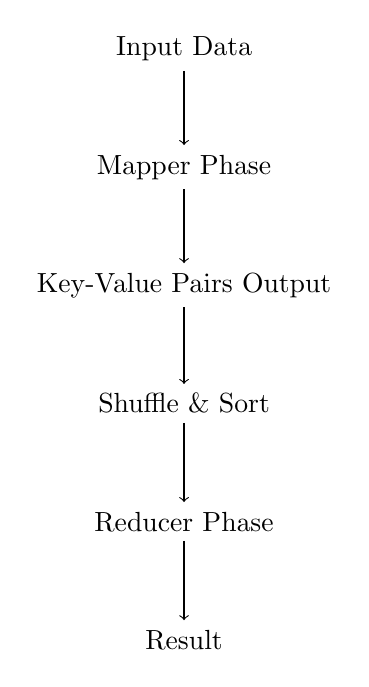
\begin{tikzpicture}
            \node (input) at (0, 0) {Input Data};
            \node (mapper) at (0, -1.5) {Mapper Phase};
            \node (kv) at (0, -3) {Key-Value Pairs Output};
            \node (shuffle) at (0, -4.5) {Shuffle \& Sort};
            \node (reducer) at (0, -6) {Reducer Phase};
            \node (result) at (0, -7.5) {Result};

            \draw[->] (input) -- (mapper);
            \draw[->] (mapper) -- (kv);
            \draw[->] (kv) -- (shuffle);
            \draw[->] (shuffle) -- (reducer);
            \draw[->] (reducer) -- (result);
        \end{tikzpicture}
    \end{center}
\end{frame}

\begin{frame}[fragile]
    \frametitle{Common Use Cases for MapReduce - Introduction}
    \begin{block}{Overview}
        MapReduce is a programming model used for processing and generating large datasets. 
        It leverages a distributed computing model, making it efficient in handling vast amounts of data across multiple nodes in a Hadoop cluster.
    \end{block}
    \begin{block}{Purpose of the Slide}
        This slide explores practical applications of MapReduce in real-world scenarios, highlighting its significance in big data processing.
    \end{block}
\end{frame}

\begin{frame}[fragile]
    \frametitle{Common Use Cases for MapReduce - Key Use Cases}
    \begin{enumerate}
        \item \textbf{Data Analysis}
        \begin{itemize}
            \item \textbf{Example:} E-commerce companies analyzing purchasing data.
            \item \textbf{Process:} 
            \begin{itemize}
                \item \textit{Map Phase:} Emit key-value pairs of customer IDs and purchase totals.
                \item \textit{Reduce Phase:} Aggregate totals to identify top customers.
            \end{itemize}
            \item \textbf{Benefit:} Helps in creating targeted marketing strategies.
        \end{itemize}
        
        \item \textbf{Log Processing}
        \begin{itemize}
            \item \textbf{Example:} Analyzing web server logs for traffic monitoring.
            \item \textbf{Process:} 
            \begin{itemize}
                \item \textit{Map Phase:} Emit key-value pairs of IP addresses and status codes.
                \item \textit{Reduce Phase:} Count occurrences of IPs and track error rates.
            \end{itemize}
            \item \textbf{Benefit:} Provides insights into website performance.
        \end{itemize}
    \end{enumerate}
\end{frame}

\begin{frame}[fragile]
    \frametitle{Common Use Cases for MapReduce - Additional Use Cases}
    \begin{enumerate}[resume]
        \item \textbf{Text Mining and NLP}
        \begin{itemize}
            \item \textbf{Example:} Analyzing documents for sentiment or keyword extraction.
            \item \textbf{Benefit:} Helps organizations analyze public sentiment towards products.
        \end{itemize}

        \item \textbf{Machine Learning Model Training}
        \begin{itemize}
            \item \textbf{Example:} Training predictive models on large datasets.
            \item \textbf{Benefit:} Efficiently processes big data for accelerated model training.
        \end{itemize}

        \item \textbf{Image Processing}
        \begin{itemize}
            \item \textbf{Example:} Analyzing images for features like facial recognition.
            \item \textbf{Benefit:} Scales analysis tasks across numerous images in a dataset.
        \end{itemize}
    \end{enumerate}
\end{frame}

\begin{frame}[fragile]
    \frametitle{Common Use Cases for MapReduce - Key Points and Conclusion}
    \begin{block}{Key Points to Emphasize}
        \begin{itemize}
            \item \textbf{Scalability:} Distributes workload to efficiently process large volumes of data.
            \item \textbf{Fault Tolerance:} Resilient to hardware failures; tasks can be redirected.
            \item \textbf{Versatility:} Applicable across industries for various data-intensive tasks.
        \end{itemize}
    \end{block}

    \begin{block}{Conclusion}
        MapReduce is a powerful tool in the Hadoop ecosystem, with versatile applications across industries. Understanding its real-world use cases emphasizes its significance in managing big data.
    \end{block}
\end{frame}

\begin{frame}[fragile]
    \frametitle{Further Exploration}
    Interested learners can explore additional components of Hadoop such as Hive and Pig. 
    These tools simplify interactions with MapReduce jobs, facilitating data queries and manipulation for users unfamiliar with programming.
\end{frame}

\begin{frame}[fragile]
    \frametitle{Challenges in Using Hadoop - Overview}
    \begin{block}{Overview}
        While Hadoop provides robust solutions for big data processing, its implementation is often accompanied by challenges. Understanding these challenges can aid organizations in strategizing and applying best practices for successful Hadoop adoption.
    \end{block}
\end{frame}

\begin{frame}[fragile]
    \frametitle{Challenges in Using Hadoop - Key Challenges}
    \begin{enumerate}
        \item \textbf{Complexity of Setup and Configuration}
            \begin{itemize}
                \item \textbf{Description:} Technically demanding to configure components (HDFS, YARN, MapReduce).
                \item \textbf{Example:} Network configuration to prevent data traffic bottlenecks.
                \item \textbf{Solution:} Use tools like Apache Ambari to simplify installation.
            \end{itemize}
        
        \item \textbf{Data Quality and Consistency}
            \begin{itemize}
                \item \textbf{Description:} Large data volumes from diverse sources may decrease quality.
                \item \textbf{Example:} Noise from log files and discrepancies from user data.
                \item \textbf{Solution:} Data validation and cleansing during ingestion.
            \end{itemize}
        
        \item \textbf{Performance Tuning and Optimization}
            \begin{itemize}
                \item \textbf{Description:} Default performance may not meet application needs.
                \item \textbf{Example:} Inefficient MapReduce jobs due to suboptimal resource allocation.
                \item \textbf{Solution:} Adjust `mapreduce.map.memory.mb` and `mapreduce.reduce.memory.mb` settings.
            \end{itemize}
    \end{enumerate}
\end{frame}

\begin{frame}[fragile]
    \frametitle{Challenges in Using Hadoop - Additional Challenges}
    \begin{enumerate}
        \setcounter{enumi}{3}
        \item \textbf{Scalability Issues}
            \begin{itemize}
                \item \textbf{Description:} Improper architecture may lead to performance drops as load increases.
                \item \textbf{Example:} Adding nodes without management can cause network overhead.
                \item \textbf{Solution:} Optimize HDFS block size configurations.
            \end{itemize}
        
        \item \textbf{Skill Shortage}
            \begin{itemize}
                \item \textbf{Description:} High demand for Hadoop experts complicates hiring.
                \item \textbf{Example:} Difficulty in finding qualified data engineers.
                \item \textbf{Solution:} Offer training and development programs for employees.
            \end{itemize}

        \item \textbf{Security Concerns}
            \begin{itemize}
                \item \textbf{Description:} Sensitive data handling raises security issues.
                \item \textbf{Example:} Potential data breaches without proper access controls.
                \item \textbf{Solution:} Implement Kerberos authentication and robust security features.
            \end{itemize}
    \end{enumerate}
\end{frame}

\begin{frame}[fragile]
    \frametitle{Challenges in Using Hadoop - Conclusion}
    \begin{block}{Conclusion}
        To effectively use Hadoop, organizations must address these challenges. Strategies such as:
        \begin{itemize}
            \item Utilizing automated setup tools
            \item Implementing data quality measures
            \item Performance tuning through adjustments
            \item Effective scaling and architecture planning
            \item Workforce training initiatives
            \item Enforcing security protocols
        \end{itemize}
        can enable a more successful Hadoop experience.
    \end{block}
\end{frame}

\begin{frame}[fragile]
    \frametitle{Challenges in Using Hadoop - Key Points}
    \begin{itemize}
        \item Understanding the complexity of Hadoop setup for smoother deployment.
        \item Prioritizing data quality for accurate analytics.
        \item Regular performance tuning to maintain efficiency.
        \item Planning for scalability to handle data growth.
        \item Investing in workforce training to bridge skill gaps.
        \item Implementing robust security measures to protect sensitive information.
    \end{itemize}
\end{frame}

\begin{frame}[fragile]
    \frametitle{Challenges in Using Hadoop - Code Snippet}
    \begin{lstlisting}[language=bash]
# Sample command to start a Hadoop daemon
$ start-dfs.sh
    \end{lstlisting}
\end{frame}

\begin{frame}[fragile]
    \titlepage
\end{frame}

\begin{frame}[fragile]
    \frametitle{Overview of Hadoop Advances}
    The Hadoop ecosystem has witnessed significant advancements aimed at enhancing performance, usability, and scalability for big data applications. 
    We will explore the latest developments, along with practical examples of how these advancements integrate into data processing workflows.
\end{frame}

\begin{frame}[fragile]
    \frametitle{1. Improved Performance with Hadoop 3.x}
    The latest Hadoop version, 3.x, comes with many performance improvements, including:
    \begin{itemize}
        \item \textbf{Erasure Coding}: Reduces storage overhead while maintaining data durability. For instance, in traditional settings, data replication requires substantial storage (3 copies by default). Erasure coding helps reduce this to 2 copies with similar reliability.
        
        \item \textbf{YARN Improvements}: Enhancements allow for better resource management and scheduling. With new optimizations, applications can experience reduced latency and increased throughput.
    \end{itemize}
\end{frame}

\begin{frame}[fragile]
    \frametitle{2. Native Support for Cloud Environments}
    Hadoop now offers native integration with cloud services, promoting flexibility and scalability:
    \begin{itemize}
        \item \textbf{Hadoop on AWS \& Azure}: Easily deploy a fully managed Hadoop cluster using services like Amazon EMR and Azure HDInsight, enabling businesses to scale up or down based on demand.
        
        \item \textbf{Data Lake Integration}: Organizations can store massive amounts of structured and unstructured data using Hadoop along with cloud services, creating a more efficient Big Data processing framework.
    \end{itemize}
\end{frame}

\begin{frame}[fragile]
    \frametitle{3. Incorporation of Machine Learning Libraries}
    Recent Hadoop distributions have integrated ML libraries, enhancing its capability to support data science applications:
    \begin{itemize}
        \item \textbf{Apache Mahout}: A scalable machine learning library that provides algorithms for clustering, classification, and collaborative filtering.
        
        \item \textbf{Apache Spark Integration}: Bundling Spark with Hadoop enhances real-time data processing, making it easier to train ML models on large datasets.
    \end{itemize}
\end{frame}

\begin{frame}[fragile]
    \frametitle{4. Enhanced Security Features}
    The push for better security measures has led to improvements such as:
    \begin{itemize}
        \item \textbf{Ranger and Knox}: These tools provide fine-grained authorization and authentication, ensuring sensitive data is secure within the Hadoop ecosystem.
        
        \item \textbf{Data Encryption}: Improved mechanisms for data encryption at rest and in transit, which are crucial for compliance in industries like finance and healthcare.
    \end{itemize}
\end{frame}

\begin{frame}[fragile]
    \frametitle{Key Points to Emphasize}
    \begin{itemize}
        \item Hadoop 3.x focuses on reduced storage costs and improved resource management.
        \item Cloud integration allows for flexibility in scaling data processing.
        \item Machine learning libraries enhance Hadoop's appeal for data-driven enterprises.
        \item Security measures are continuously evolving to protect against data breaches.
    \end{itemize}
\end{frame}

\begin{frame}[fragile]
    \frametitle{Conclusion}
    Hadoop continues to evolve, meeting the demands of modern data processing needs. By embracing these advancements, organizations can enhance their data processing capabilities, ensuring efficient and secure handling of big data.
\end{frame}

\begin{frame}[fragile]
    \frametitle{Conclusion - Overview of the Hadoop Ecosystem}
    \begin{block}{Hadoop Ecosystem Overview}
        The Hadoop Ecosystem comprises a suite of tools and technologies that support the storage, processing, and analysis of large data sets. 
        It is vital in the era of big data due to its:
        \begin{itemize}
            \item Ability to scale effectively
            \item Efficient data management
            \item Processing of complex datasets
        \end{itemize}
    \end{block}
\end{frame}

\begin{frame}[fragile]
    \frametitle{Conclusion - Key Components}
    \begin{block}{Key Components of the Hadoop Ecosystem}
        \begin{enumerate}
            \item \textbf{HDFS (Hadoop Distributed File System)}
            \begin{itemize}
                \item Scalable file storage system across clusters.
                \item Example: Companies like Facebook and Twitter manage petabytes of user data with HDFS.
            \end{itemize}
            
            \item \textbf{MapReduce}
            \begin{itemize}
                \item Programming model for distributed data processing.
                \item Example: Analyzing customer purchase patterns to extract marketing insights.
            \end{itemize}
            
            \item \textbf{YARN (Yet Another Resource Negotiator)}
            \begin{itemize}
                \item Manages resources for multiple data processing engines.
                \item Example: Dynamically allocating resources for different jobs.
            \end{itemize}
            
            \item \textbf{Ecosystem Tools}
            \begin{itemize}
                \item Apache Hive, Apache Pig, Apache HBase, Apache Spark
            \end{itemize}
        \end{enumerate}
    \end{block}
\end{frame}

\begin{frame}[fragile]
    \frametitle{Conclusion - Importance and Application}
    \begin{block}{Importance of Hadoop Ecosystem}
        \begin{itemize}
            \item \textbf{Scalability:} Easily scales horizontally to handle rapid data growth.
            \item \textbf{Cost-Effectiveness:} Utilizes commodity hardware for reduced storage costs.
            \item \textbf{Flexibility:} Handles structured, semi-structured, and unstructured data.
        \end{itemize}
    \end{block}

    \begin{block}{Real-World Applications}
        \begin{itemize}
            \item \textbf{Healthcare:} Analytics for improved patient outcomes.
            \item \textbf{Finance:} Risk analysis and fraud detection in real-time.
            \item \textbf{Retail:} Optimizing inventory management and customer analytics.
        \end{itemize}
    \end{block}
    
    \begin{block}{Key Takeaway}
        The Hadoop Ecosystem is integral to the big data landscape, enabling efficient, scalable, and flexible data processing solutions for informed decision-making.
    \end{block}
\end{frame}


\end{document}